%----------------------------------------------------------------------------------------
%   SECTION 3: TRAJECTORY GENERATION
%----------------------------------------------------------------------------------------

\section{Task 2: Trajectory Generation (Newton's Method)}

To generate feasible trajectories transitioning between system equilibria, we employed a Newton-type method for optimal control, specifically a Differential Dynamic Programming (DDP) approach. This method iteratively optimizes the control sequence by utilizing quadratic approximations of the cost function and linear approximations of the system dynamics to find a local minimum of the objective function.

\subsection{Reference Generation}
Given the non-convex nature of the optimization landscape, the solver requires a reasonable reference trajectory to guide convergence, even if that reference is dynamically infeasible. We analyzed two distinct generation methods:

\begin{enumerate}
    \item \textbf{Stepwise:} A naive approach involving an instantaneous switch from the initial state $x_{start}$ to the goal state $x_{goal}$. This introduces a large discontinuity in the error term, often leading to poor convergence or aggressive control spikes.
    \item \textbf{Polynomial Interpolation (Poly 5):} We generated smooth references for joint positions and velocities using 5th-order polynomials. This method ensures kinematic consistency by respecting boundary conditions (position, velocity), thereby significantly aiding the solver in finding a feasible solution.
\end{enumerate}

\begin{figure}[H]
    \centering
    % First Subfigure
    \begin{subfigure}[b]{0.8\textwidth}
        \centering
        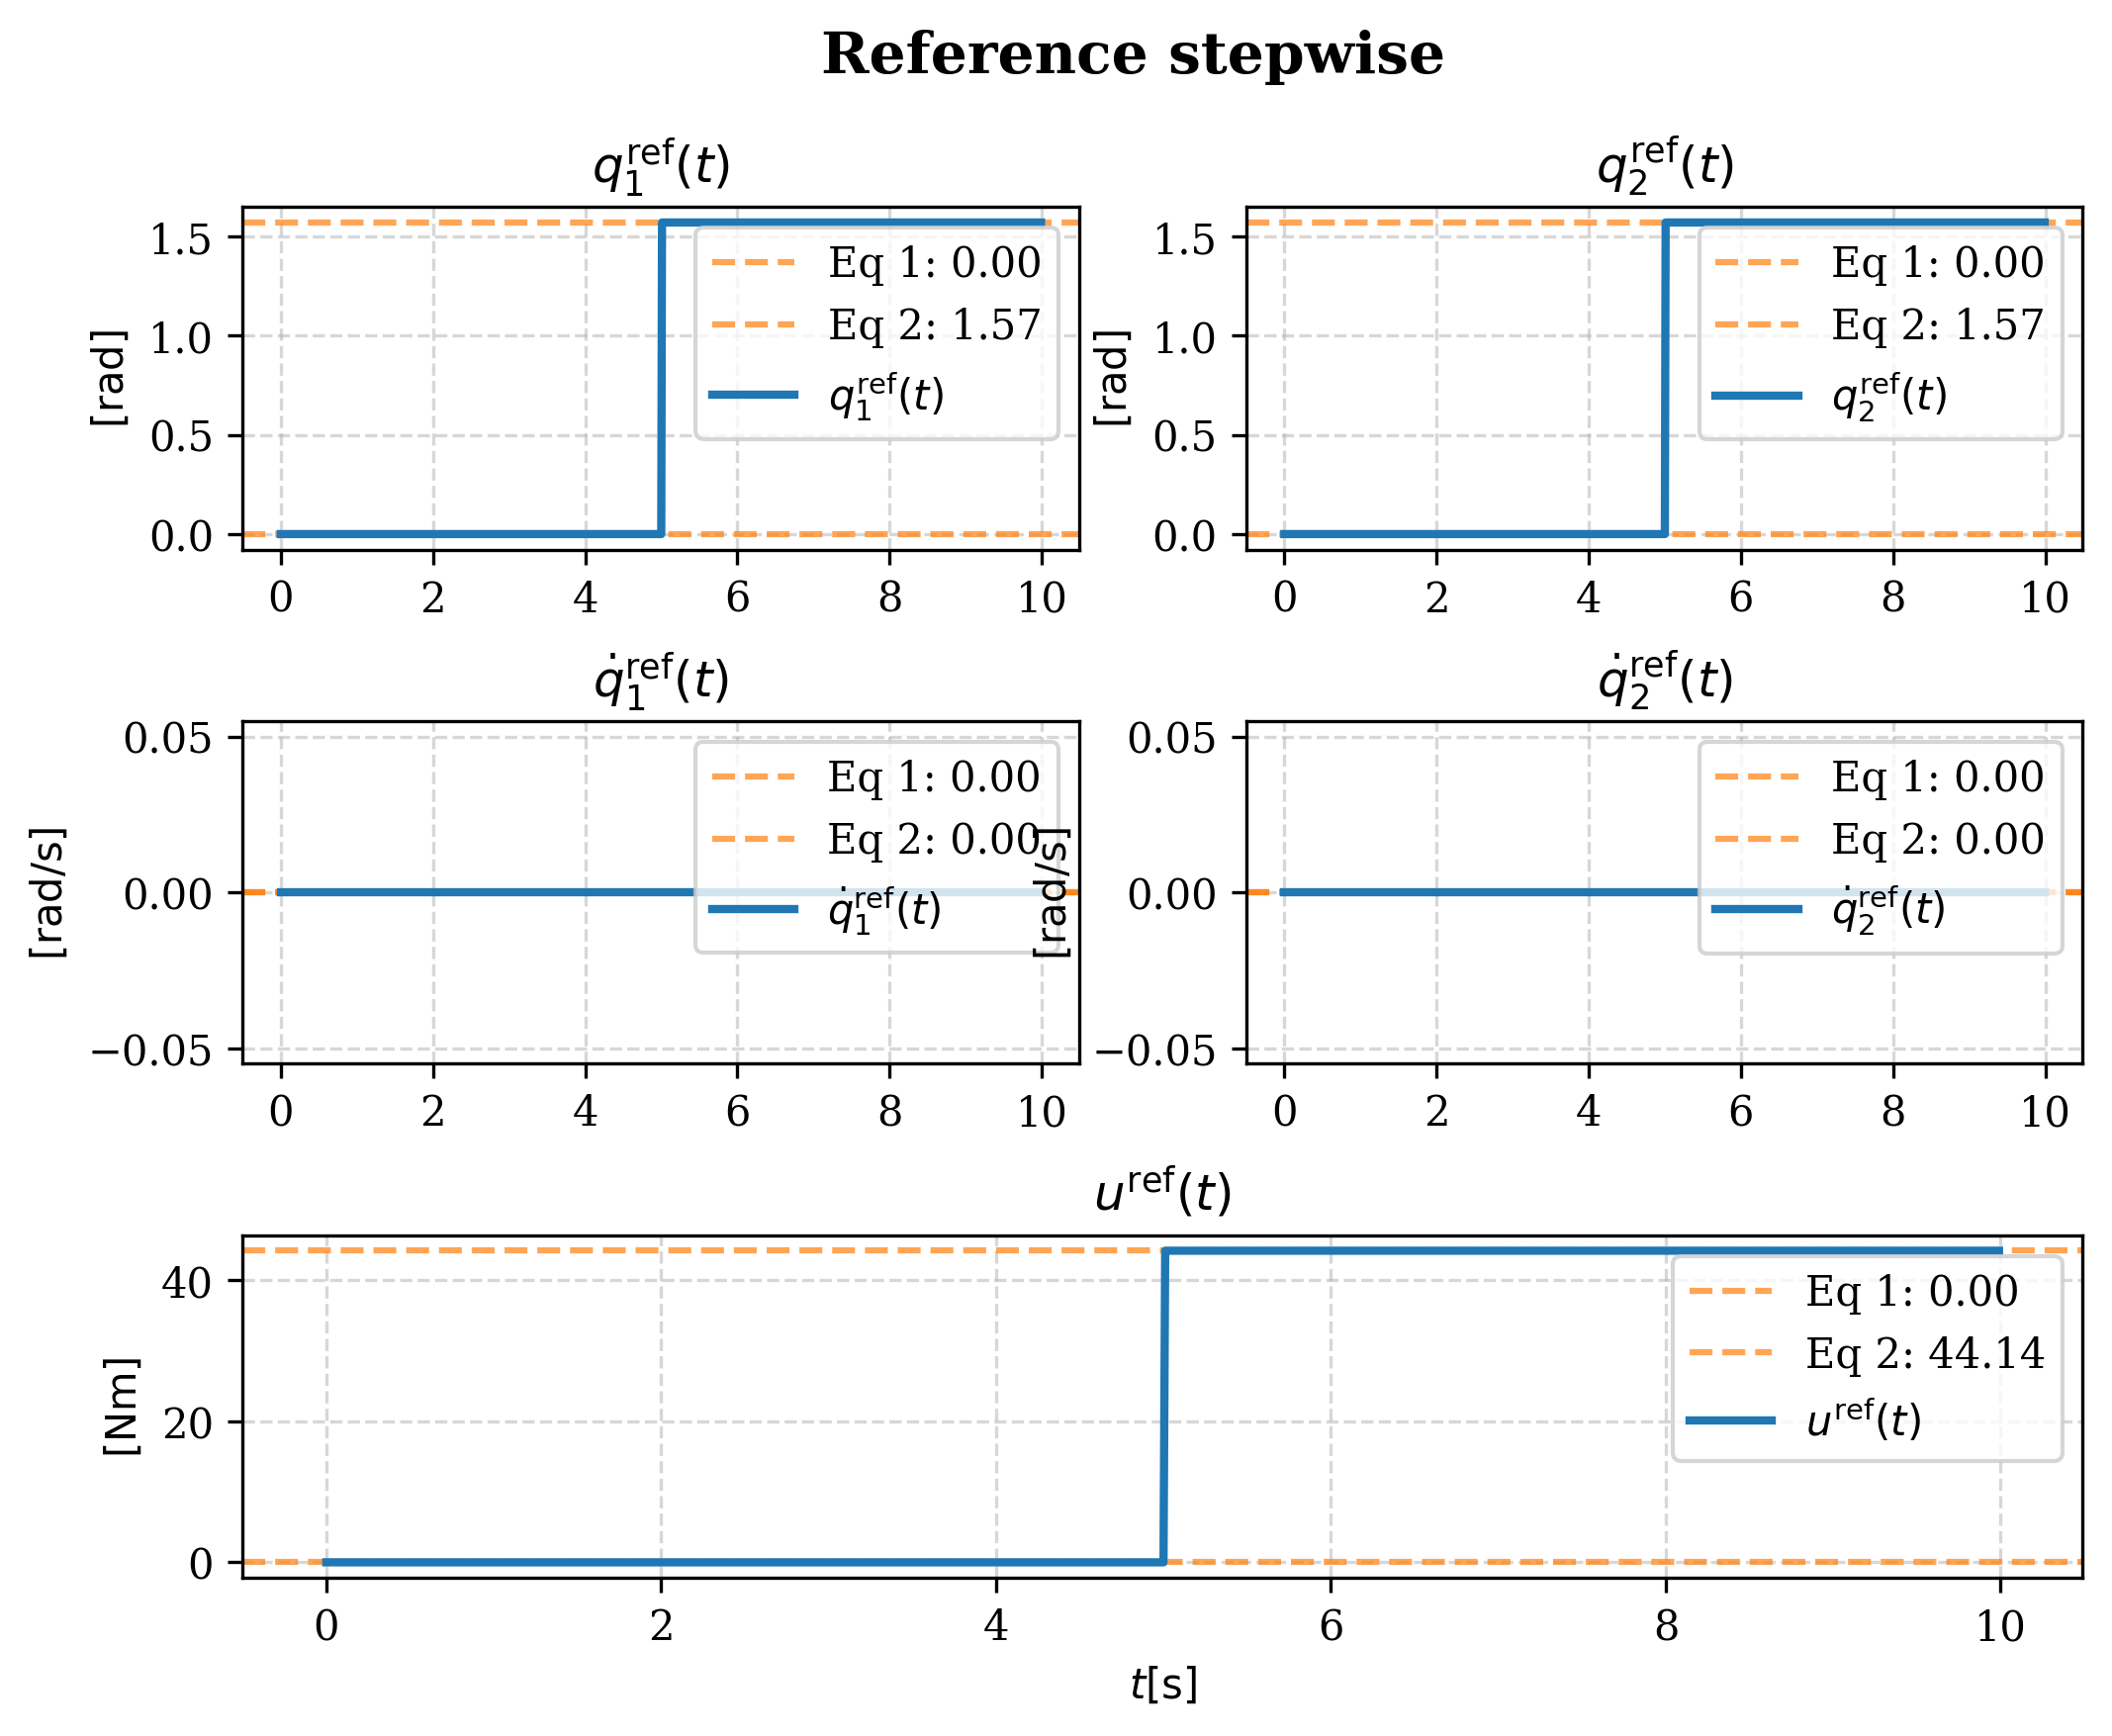
\includegraphics[width=\linewidth]{figs/misc/reference_trajectory.png}
        \caption{Stepwise Reference}
        \label{fig:ref_stepwise}
    \end{subfigure}

    \caption{Comparison of reference generation strategies.}
    \label{fig:reference_comparison}
\end{figure}


\begin{figure}[H]
    \ContinuedFloat % This command links this figure to the previous one
    \centering
    % Second Subfigure
    \begin{subfigure}[b]{0.8\textwidth}
        \centering
        \includegraphics[width=\linewidth]{figs/branch4/traj_gen_newton/elbow_up/reference_trajectory.png}
        \caption{Poly 5 Reference}
        \label{fig:ref_poly5}
    \end{subfigure}
\end{figure}


\subsubsection{Task Definitions}
We defined a set of standard maneuvers of varying complexity to evaluate the generation algorithms, ranging from simple transitions to complex swings.

\begin{figure}[H]
    \centering
    \begin{subfigure}[b]{0.5\textwidth}
        \centering
        \includegraphics[width=\linewidth]{figs/branch4/traj_gen_newton/elbow_up/double_pendulum_envelope.png}
        \caption{Elbow Up}
        \label{fig:task_elbowup}
    \end{subfigure}
    
     \begin{subfigure}[b]{0.5\textwidth}
        \centering
        \includegraphics[width=\linewidth]{figs/branch4/traj_gen_newton/swing_up/double_pendulum_envelope.png}
        \caption{Swing Up}
        \label{fig:task_swingup}
    \end{subfigure}
    
    \caption{Visualization of the defined control tasks and their target equilibria.}
\end{figure}
\begin{figure}[H]
    \centering
    \begin{subfigure}[b]{0.5\textwidth}
        \centering
        \includegraphics[width=\linewidth]{figs/branch4/traj_gen_newton/swing_down/double_pendulum_envelope.png}
        \caption{Swing Down}
        \label{fig:task_swingdown}
    \end{subfigure}
    
    \begin{subfigure}[b]{0.5\textwidth}
        \centering
        \includegraphics[width=\linewidth]{figs/branch4/traj_gen_newton/complex_maneuver/double_pendulum_envelope.png}
        \caption{Complex Maneuver}
        \label{fig:task_complex}
    \end{subfigure}
    x
    \label{fig:tasks}
\end{figure}

\subsection{Performance Analysis: Stepwise vs. Polynomial}

The choice of reference trajectory significantly impacts the solver's performance. When applying Newton's method to the \textbf{Stepwise} reference, we observed significant limitations. As seen in Figure \ref{fig:newton_stepwise}, the instantaneous jump in the reference creates a large error gradient at the transition point. The solver attempts to compensate with an infeasible spike in control torque $u$, often pushing the system into unstable regions.

\begin{figure}[H]
    \centering
    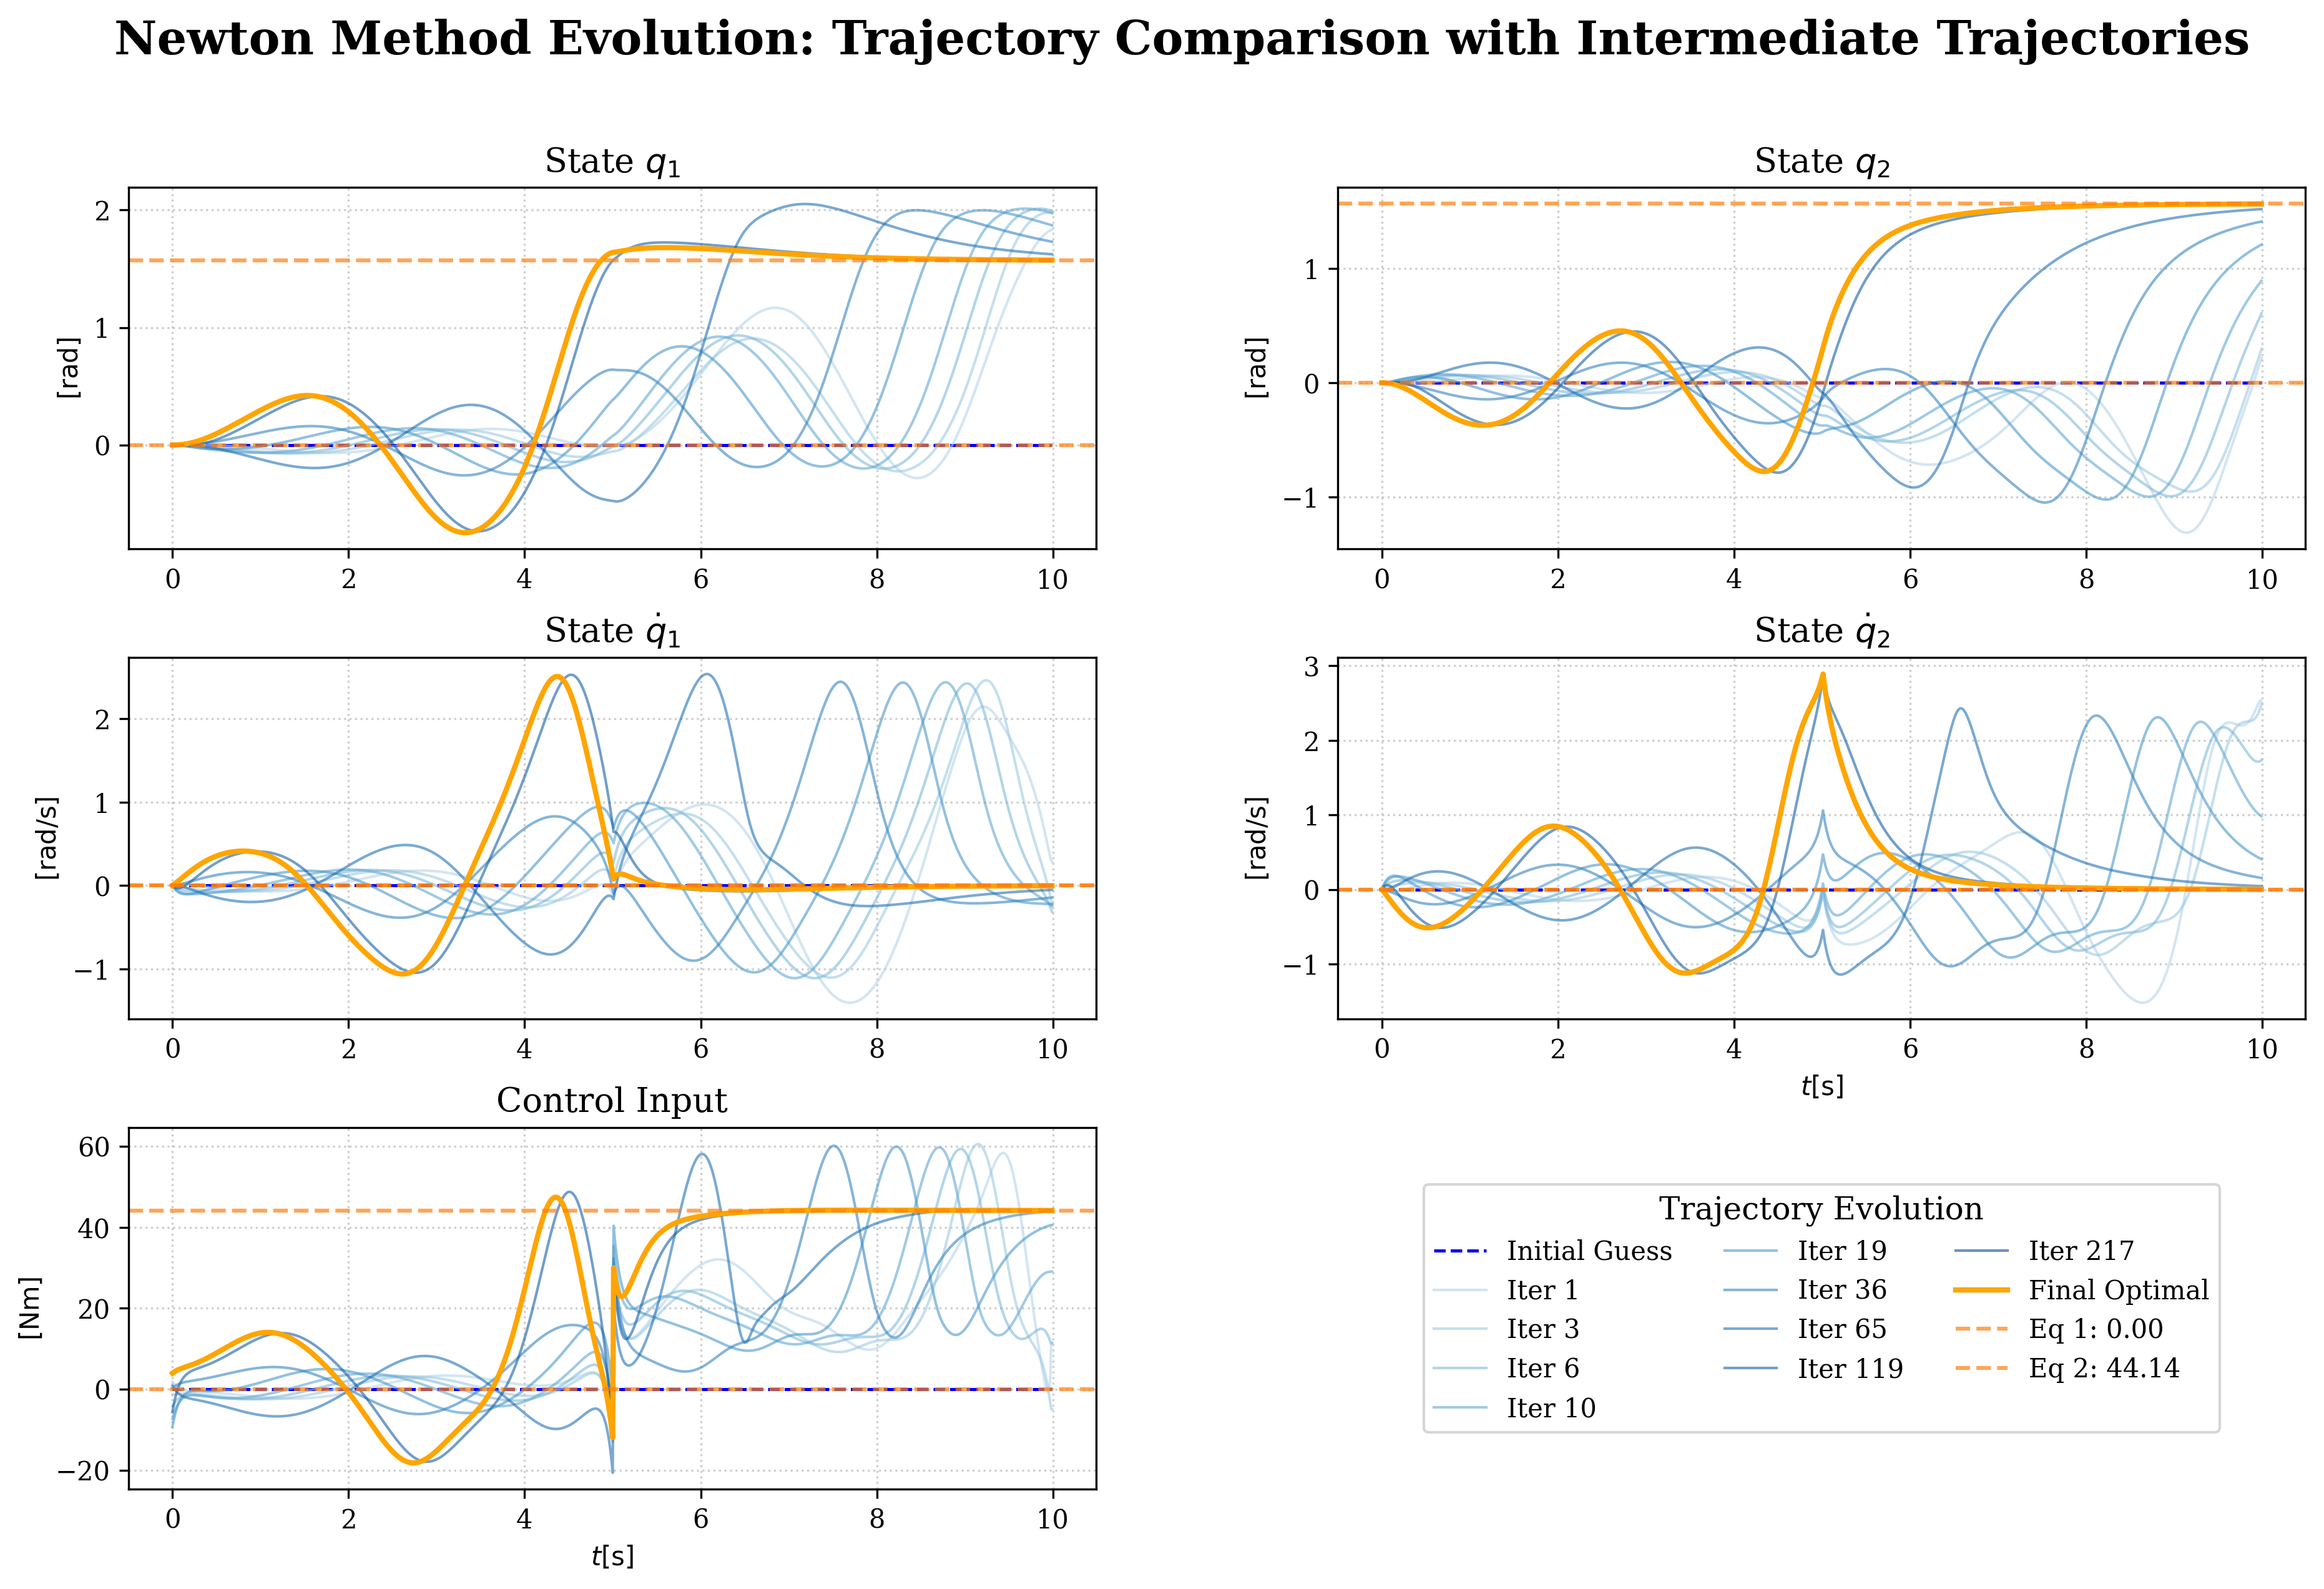
\includegraphics[width=0.8\linewidth]{figs/misc/trajectory_comparison_mid.png}
    \caption{Newton's method applied to Elbow Up using Stepwise reference. Note the control discontinuity.}
    \label{fig:newton_stepwise}
\end{figure}

Conversely, the \textbf{Polynomial (Poly 5)} reference provides a physically plausible kinematic guide. However, physical constraints inherent to the under-actuated flexible link still present challenges:

\begin{itemize}
    \item \textbf{Energy Transfer (Elbow Up):} During swing-up motions, kinetic energy must be efficiently transferred to potential energy. The polynomial reference guides this transfer smoothly.
    \item \textbf{Energy Dissipation (Elbow Down):} In downward motions, the passive second link cannot be directly braked. Since the system friction is low, the controller cannot rely on passive dissipation; it must actively pump energy out of the system via dynamic coupling. This becomes infeasible if the reference demands a deceleration rate faster than the system's natural dynamics allow.
\end{itemize}

\begin{figure}[H]
    \centering
    \begin{subfigure}[b]{0.8\textwidth}
        \centering
        \includegraphics[width=\linewidth]{figs/branch4/traj_gen_newton/swing_up/trajectory_comparison_mid.png}
        \caption{Poly 5 applied to Swing Up}
        \label{fig:newton_poly_up}
    \end{subfigure}
    \hfill
    \begin{subfigure}[b]{0.8\textwidth}
        \centering
        \includegraphics[width=\linewidth]{figs/branch4/traj_gen_newton/the_dive/trajectory_comparison_mid.png}
        \caption{Poly 5 applied to Swing Down}
        \label{fig:newton_poly_down}
    \end{subfigure}
    \caption{Optimization results using 5th-order polynomial references.}
    \label{fig:newton_poly_results}
\end{figure}

\subsection{Optimization Challenges}
Applying the standard Newton method directly to complex, long-horizon maneuvers revealed several critical numerical and theoretical issues:

\begin{itemize}
    \item \textbf{Non-Convex Optimization Landscape:} The trajectory manifold for complex maneuvers is highly non-linear, and the cost landscape is riddled with local minima. If the initial guess falls within the basin of attraction of a local minimum—representing a partial swing or a stalled state—the solver is unable to escape to the global optimum.
    
    \item \textbf{Long Time Horizons and Sensitivity:} Extending the time horizon $T$ exponentially increases the complexity of the solution space. Conversely, a long horizon increases the condition number of the Hessian matrix. Small changes in initial inputs propagate through the sensitivity matrix $\prod_{k=0}^{T-1} A_k$, causing massive deviations in terminal states and leading to numerical divergence.

    \item \textbf{Fixed Horizon Inflexibility:} A significant limitation of standard DDP is the rigidity of the fixed time horizon. If the chosen $T$ is mismatched with the natural frequency of the maneuver, the optimization may be physically impossible to solve, leading to poor convergence.

    \item \textbf{Controllability and Terminal Cost:} Implementing a stabilizing terminal cost $Q_T$ requires solving the Discrete Algebraic Riccati Equation (DARE). This necessitates that the system linearization $(A, B)$ at the target equilibrium be stabilizable. In under-actuated configurations, kinematic singularities can cause rank deficiencies in the controllability matrix, rendering the DARE unsolvable.

    \item \textbf{Instability to Dwell Time:} We observed numerical instability when requiring the system to maintain an unstable equilibrium for a final time interval (dwell time). Any numerical error $\epsilon$ at $t < T$ is amplified by the unstable eigenvalues of the system evolution matrix ($A^k$). This creates a "narrow ridge" in the cost landscape where slight deviations result in massive penalties.

    \item \textbf{Linearization Validity:} The optimization relies on linearizing the non-linear dynamics around the current trajectory. If the update step is too large, the Taylor approximation breaks down, leading to valid descent directions becoming actual ascent directions in the true non-linear landscape.
\end{itemize}

\subsubsection{Visual Analysis of the Local Minimum Trap}
The issue of local minima is illustrated in Figure \ref{fig:optimal_trajectory_suboptimal}. Despite starting with a reasonable guess, the intermediate iterations cluster around a suboptimal path, and the optimization fails to reach the final equilibrium.

\begin{figure}[H]
    \centering
    \includegraphics[width=1.0\linewidth]{figs/branch4/traj_gen_newton/custom5/trajectory_comparison_mid.png}
    \caption{Illustration of the "Local Minimum Trap" where the solver converges to a suboptimal trajectory rather than the target equilibrium.}
    \label{fig:optimal_trajectory_suboptimal}
\end{figure}

Crucially, standard convergence metrics can be misleading in this scenario. Figures \ref{fig:cost_function_complex} and \ref{fig:descent_complex} show that the cost function plateaus to a finite value and the descent direction norm approaches zero. This indicates that the solver has successfully found a mathematical minimum (gradient is zero), but it is a local minimum that fails to satisfy the physical task requirements. Nominal convergence does not imply task success.

\begin{figure}[H]
    \centering
    \includegraphics[width=0.8\linewidth]{figs/branch4/traj_gen_newton/custom5/cost_function.png}
    \caption{Cost function evolution during failure. The cost converges to a steady value, concealing the failure to reach the target.}
    \label{fig:cost_function_complex}
\end{figure}

\begin{figure}[H]
    \centering
    \includegraphics[width=0.8\linewidth]{figs/branch4/traj_gen_newton/custom5/descent_direction.png}
    \caption{Descent direction norm. The algorithm mathematically converges (norm $\to 0$), but to an incorrect solution.}
    \label{fig:descent_complex}
\end{figure}

\subsection{Proposed Solution: Dynamic Horizon Extension}

To address the ill-conditioning and local minima problems described previously, we implemented a \textbf{Dynamic Horizon Extension} strategy. Instead of attempting to solve the optimization problem for the full duration $T_{final}$ immediately, we solve a sequence of sub-problems with incrementally increasing horizon lengths. This strategy effectively conditions the optimization by ensuring the solver always operates within a valid local approximation of the system dynamics.

\subsubsection{Theoretical Justification}
\begin{enumerate}
    \item \textbf{Conditioning:} For a short horizon $T$, the norm of the sensitivity matrix ($\prod A_t$) remains bounded. This results in a well-conditioned Hessian and a significantly larger basin of attraction for Newton's method.
    \item \textbf{Warm Starting:} The optimal solution derived for horizon $T$ serves as the initial guess for the extended horizon $T + \Delta T$. This "anchors" the subsequent optimization in a feasible region of the state space, maintaining proximity to physical constraints.
    \item \textbf{Iterative Refinement:} As the horizon expands, the solver's task is reduced to refining the control inputs locally rather than discovering a global solution from scratch. This prevents the explosive divergence typically associated with global searches in ill-conditioned landscapes.
\end{enumerate}

\subsubsection{Algorithm Implementation}
The iterative procedure is defined as follows:
\begin{enumerate}
    \item \textbf{Initialize:} Set a short initial horizon $T_{curr} \ll T_{final}$ such that the DARE-based terminal cost effectively approximates the remaining cost-to-go.
    \item \textbf{Converge:} Execute the Newton solver until the optimality criteria (gradient norm close to zero) are met for the current $T_{curr}$.
    \item \textbf{Extend:} Use the computed trajectory $x^*(t)$ as the initial guess for the next phase. The horizon is extended by $\Delta T$, and the reference tail is padded with the target equilibrium. The initial guess for the new segment is generated by evolving the system dynamics forward from the previous terminal state.
    \item \textbf{Repeat:} Increment $T_{curr} \leftarrow T_{curr} + \Delta T$ and repeat the process until $T_{curr} \geq T_{final}$ and the terminal error satisfies $\|\mathbf{x}_T - \mathbf{x}_{target}\| < \epsilon$.
\end{enumerate}

\subsubsection{Numerical Analysis and Validation}

The efficacy of the Dynamic Horizon Extension is visually demonstrated in the evolution of the system trajectories and optimization metrics.

\begin{figure}[H]
    \centering
    \includegraphics[width=1.0\linewidth]{figs/branch5/traj_gen_newton/custom5/trajectory_comparison_mid_extended.png}
    \caption{Evolution of the trajectory during the Dynamic Horizon Extension process. The system incrementally "learns" the complex maneuver.}
    \label{fig:horizon_extension}
\end{figure}

Figure \ref{fig:horizon_extension} illustrates the iterative learning process for a complex maneuver. Initially, the optimization explores suboptimal paths restricted by the short time horizon. As the horizon extends, the solver progressively uncovers the feasible manifold, guiding the trajectory into a "narrow channel" of state space that leads precisely to the unstable equilibrium. The abrupt changes in trajectory shape between phases indicate the solver escaping local basins of attraction that would otherwise trap a static-horizon optimization.

\begin{figure}[H]
    \centering
    \includegraphics[width=0.8\linewidth]{figs/branch5/traj_gen_newton/custom5/cost_function.png}
    \caption{Step-wise evolution of the cost function. Each "step" corresponds to a horizon extension.}
    \label{fig:horizon_extension_cost}
\end{figure}

\begin{figure}[H]
    \centering
    \includegraphics[width=0.8\linewidth]{figs/branch5/traj_gen_newton/custom5/descent_direction.png}
    \caption{Norm of the descent direction. Spikes indicate the start of a new extension phase, followed by rapid convergence.}
    \label{fig:horizon_extension_descent}
\end{figure}

This behavior is further corroborated by the cost function evolution shown in Figure \ref{fig:horizon_extension_cost}. It is observed that earlier, shorter solutions yield a lower total cumulative cost than the final "correct" solution. This result highlights the regularizing effect of the algorithm: a direct full-horizon optimization would likely converge to a lower-energy, locally optimal solution (like a partial swing) that fails to reach the target. By incrementally extending the horizon, we force the system to accept a higher-cost trajectory that satisfies the terminal boundary conditions.

The descent direction norm (Figure \ref{fig:horizon_extension_descent}) confirms the stability of this approach. Each horizon extension introduces a perturbation, visible as a spike in the descent magnitude. However, because the system is warm-started from a feasible prior solution, the solver rapidly reconverges (descent norm $\to 0$) within a few iterations. This proves that the algorithm successfully transforms a difficult global search into a series of manageable local refinements.
\pagebreak


 % \item \textbf{Ill-Conditioning of the Hessian}:

% Newton's method updates the control sequence by solving a linear system involving the Hessian of the cost function, $H$. The step $\Delta \mathbf{u}$ is calculated as:

% \begin{equation}

% \Delta \mathbf{u} = -H^{-1} g

% \end{equation}

% where $g$ is the gradient. As $N$ increases, the massive magnitude disparity in the sensitivity matrix $A^N$ causes the condition number of the Hessian,

% $\kappa(H) = \frac{|\lambda_{\max}|}{|\lambda_{\min}|}$, to skyrocket. This leads to the following effect: infinitesimal changes in the inputs (especially first ones) imply massive

% changes in $x_N$, causing the Newton step to overshoot local minima and resulting in numerical divergence.

% could it be that constraining the input to stand still in the beginning we are losing our opportunity to control the unstable modes?



% \subsection{The PBH Test}

% While standard controllability checks the rank of the Kalman controllability matrix $[B, AB, \dots, A^{n-1}B]$, numerical conditioning is better assessed via the Popov-Belevitch-Hautus (PBH) test. A system is stabilizable if and only if:

% \begin{equation}

% \text{rank}([\lambda I - A \mid B]) = n \quad \forall \lambda \in \mathbb{C}, \quad |\lambda| \ge 1

% \end{equation}

%In underactuated systems (our case), kinematic singularities can cause this rank to drop (in our case we control only through coupling!). If the rank deficiency occurs at an unstable eigenvalue, the mode is \textit{uncontrollable} and \textit{unstable}. In such configurations, the Hessian becomes singular, and the Newton step is undefined.


